\section{Introduction}\label{sec:introduction}


% use cases: multi-threaded app (RSS(HW) or RPS (SW)), cloud + cluster, job queues

% moore

% embarrassingly parallel

% amdahl limits

% superlinearity observed + perpeetum motion

% we show a systematic way to architect distributed systems to achieve SL scaling: LB-LB + SA

% sims + case study - results (360x in sims, 100x in benchmarks over Linux default)

% goals/nongoals

With the end of Moore's law, computing power in modern computing systems increasingly comes in the form of parallel processing resources.  A major obstacle faced by network engineers is how to harness this increasingly parallel computing power \cite{265065, 10.5555/3307441.3307467, 10.1145/2815400.2815423, 10.1145/3098822.3098826, 10.5555/3154630.3154639}.

In horizontally scaled applications, a load balancer dispatches jobs across a fleet of workers that process the jobs in parallel \cite{10.5555/3235491}, optionally synchronizing on shared state maintained in global storage.  In the context of \emph{web applications}, HTTP load balancers \cite{194966, 211279, 9552525} distribute requests across a swarm of backend web servers by hashing over the source IP address (``sticky sessions''). This way, requests from the same client will hit the same backend server, improving request locality and hence, performance. % Meanwhile, resource state is maintained in a key-value store or a relational database.
Multicore \emph{OS network stacks} \cite{211263, 10.1145/3359989.3365412, 10.1145/3452296.3472914} leverage the NIC to dispatch packets across the CPU cores. In order to avoid packet reordering and improve CPU cache performance, load balancing typically occurs by the NIC computing a hash over the packet header, e.g., the IP 5-tuple (RSS, RPS, etc.).  In massive-scale \emph{key-value stores} \cite{ghigoff2021bmc}, the key-space is hashed into multiple shards (partitions) and each shard is assigned to a separate server. Queries are distributed over the shards by hashing the requested key, and each shard processes only a portion of the key space.

The distributed system's overall goal is to achieve the greatest possible parallel speedup in terms of the the lowest time for executing a single task or the most tasks that can be finished during a given time period. Suppose a web app handles 100 requests per second using a single server. As we add another server, we expect a throughput of 200 requests per second. In reality, however, we usually obtain slightly less, and this is worsened as the system is scaled up further. This is because some fraction of most systems is inherently sequential and, therefore, bound to execute on a single CPU core. For instance, the web server replicas may need to synchronize write access to global state in a shared data store that cannot be scaled.  Beyond a certain threshold, parallel performance plateaus due to the sequential workload becoming a bottleneck.

The maximum speedup, measured as the ratio of the wall clock times of sequential and parallel execution, is formally described by Amdahl's law \cite{10.1145/1465482.1465560}. In general, the greater the serial portion $s$ compared to the parallelizable fraction of the code, the more performance is lost compared to an ``ideal'' linear scaling and the faster the system reaches saturation (see Fig.~\ref{fig:amdahl}). Amdahl's law is a cornerstone result in the parallel and high-performance computing practice and, despite often being debated \cite{10.1145/42411.42415}, extended \cite{4563876, 6280307,1580395,406581,6163449}, and misused \cite{10.5555/775339.775386}, it has remained one of the most useful tools in the system engineering toolbox \cite{10.5555/1951599}.

\begin{figure}[t]
  \centering
  % \includegraphics[width=0.8\linewidth]{fig/usl.png}
  \begin{small}
  \begin{small}
  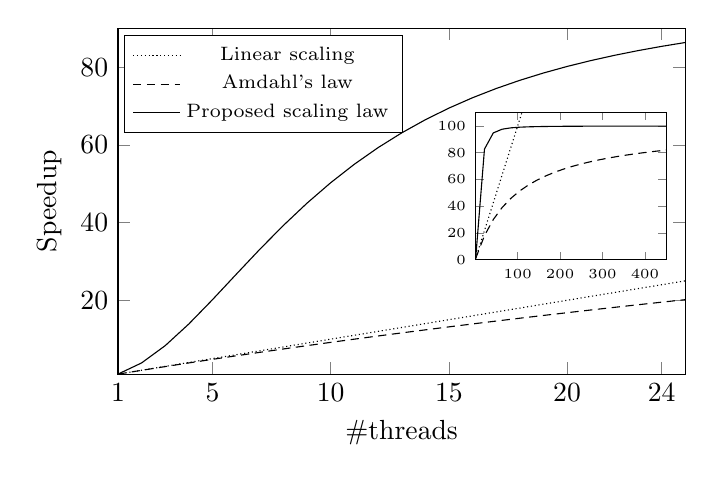
\begin{tikzpicture}[remember picture]
    \begin{axis}[
      width=250pt,
      height=170pt,
      xlabel={\#threads},
      ylabel={Speedup},
      xlabel near ticks,
      ylabel near ticks,
      xmin=1,
      xmax=25,
      ymin=1,
      ymax=90,
      xtick={1,5,10,15,20,24},
      legend style = {
        anchor = north west,
        at = {(rel axis cs:0.01,0.98)},
        font=\scriptsize,
        % draw = none,
      },
      no markers
      ]
      % use TeX as calculator:
      \addplot[domain=1:25,black,densely dotted]{x};
      \addlegendentry{Linear scaling}

      \addplot[domain=1:25,black,densely dashed]{1/(0.01 + (1-0.01)/x)};
      \addlegendentry{Amdahl's law}

      \addplot[domain=1:25,black,solid]{1/(0.01 + (1-0.01)/x^2)};
      \addlegendentry{Proposed scaling law}

      \coordinate (insetPosition) at (rel axis cs:.97,0.25);
      % \addplot[domain=0:15,black,loosely dashed]{1/(0.4 + (1-0.4)/x)};
      % \addlegendentry{Amdahl's law ($\delta=0.4$)}

      % \addplot[domain=0:15,black,loosely dotted]{1/(0.4 + (1-0.4)/x^2)};
      % \addlegendentry{Proposed scaling law for MTF ($\delta=0.4$)}
    \end{axis}
    \begin{axis}[
      at={(insetPosition)},
      anchor={outer south east},
      width=105pt,
      height=85pt,
      tiny,
      % xlabel={\#cores},
      % ylabel={Speedup},
      xmin=1,
      xmax=450,
      ymin=0,
      ymax=110,
      % ytick={1,2,3,4,5},
      no markers]
      \addplot[domain=1:500,black,densely dotted]{x};
      \addplot[domain=1:500,black,densely dashed]{1/(0.01 + (1-0.01)/x)};
      \addplot[domain=1:500,black,solid]{1/(0.01 + (1-0.01)/x^2)};
    \end{axis}
  \end{tikzpicture}
\end{small}

%%% Local Variables:
%%% mode: latex
%%% TeX-master: "../distributed_mrf.tex"
%%% End:

\end{small}
  \caption{Linear scaling, Amdahl's law and the proposed scaling law ($s=0.01$). The inset shows the asymptotics.}
  \label{fig:amdahl}
\end{figure}

Inherent to Amdahl's law is that no system can scale faster than linear: doubling parallel resources will yield at most two times the performance. Curiously, there have been several genuine experimental reports of faster-than-linear (\emph{superlinear}) scaling exhibited by various distributed applications, including databases \cite{scalability-analyzed, 10.5555/1012889.1012894}, SDN analytics \cite{sdn-analytitcs}, high-performance computing \cite{556383, 7733347}, and multi-robot systems \cite{10.1007/978-3-319-77610-1}. In general, there seem to be two ways to ways to achieve superlinear scaling \cite{7733347, 80148}: do disproportionately less work in each worker as we scale the system \cite{7733347}, or add more resources per thread \cite{80148}. One typical example for the latter case is caching \cite{271208, 10.5555/1012889.1012894}: the more CPU cores the more (unshared) L1 cache space, which tends to make memory-bound\slash cache-bound applications disproportionately faster since the application now runs on a ``Bigger Machine'' \cite{80148} (see analysis in \S\ref{sec:background}).  Many authors, however, consider this phenomenon too elusive to be exploiting in engineering general distributed applications \cite{gunther-hotsos, 10.1145/2773212.2789974, 7733347, 80148}, or outright dismiss superlinear scaling all together \cite{gunther-hotsos}, concluding that ``superlinearity, although alluring, is as illusory as perpetual motion'' \cite{10.1145/2773212.2789974}.


In parallel computing, an embarrassingly parallel workload or problem (also called embarrassingly parallelizable, perfectly parallel, delightfully parallel or pleasingly parallel) is one where little or no effort is needed to separate the problem into a number of parallel tasks.[1] This is often the case where there is little or no dependency or need for communication between those parallel tasks, or for results between them.[2] 

goals:

\begin{itemize}
\item remove the misconception that linear scaling is the best one can achieve
\item general architecture
\end{itemize}


nongoals:

\begin{itemize}
\item present the fastest available packet classifier (but results speak forthemselves)
\end{itemize}

contributions:



%%% Local Variables:
%%% mode: latex
%%% TeX-master: "distributed_mrf"
%%% End:

